\documentclass[11pt]{article} %%%%%%%%%%%%%%%%%%%%%%%%%%%

%%%%%%%%%%%%%%%%%%%%%%%%%%%%%%%%%%%%%%%%%%%%%%%%%%%%%%%%% 
%%%
%%% Blank Sweave Document
%%%   This uses xelatex and MinionPro. Most users will need
%%%   to comment out stuff in the 'fonts' section below.
%%%   It should compile in regular pdflatex, if you comment
%%%   out xltxtra and fontspec.
%%% also, you probably need to comment out \usepackage{Sweave}
%%%   to allow R to insert its own ugly default one.
%%% 
%%% mjm / 2009-11-23 %%%%%%%%%%%%%%%%%%%%%%%%%%%%%%%%%%%%


%%% options to change font. If you want to play with MinionPro,
%%% come bug me sometime. --mike
%%% LOTS OF COOL FONT INFO AT http://www.tug.dk/FontCatalogue/
%%% NO NEED EVER TO USE COMPUTER MODERN, AN ABOMINATION
%%% see also http://nitens.org/taraborelli/latex and
%%% http://scripts.sil.org/XeTeX
%\usepackage{times}
%\usepackage{cmbright}
%\renewcommand\sfdefault{phv}% use helvetica for sans serif
%\renewcommand\familydefault{\sfdefault}% use sans serif by default
\usepackage[dvipsnames,usenames]{xcolor}
%\usepackage[opticals,medfamily,minionint,footnotefigures]{MinionPro}
\usepackage[no-math]{fontspec}
\usepackage{ucs}
\usepackage[utf8]{inputenc}
\usepackage{xltxtra}
%\VignetteIndexEntry{MRP Primer Reloaded}


%%%Set up bold Minion Pro math
% \usepackage{bm}
% \DeclareMathAlphabet\mathbf {T1} {MinionPro-OsF}{b}{n}
% \SetMathAlphabet\mathit  {bold}{T1} {MinionPro-OsF}{b}{it}
% \SetSymbolFont{operators}{bold}{T1} {MinionPro-OsF}{b}{n}
% \SetSymbolFont{letters}  {bold}{OML}{MinionPro-TOsF} {b}{it}
% \DeclareMathVersion{boldtabular}
% \SetSymbolFont{operators}{boldtabular}{T1} {MinionPro-OsF}{b}{n}
% \SetSymbolFont{letters}  {boldtabular}{OML}{MinionPro-TOsF}  {b}{it}
% \SetMathAlphabet\mathit  {boldtabular}{T1} {MinionPro-OsF}{b}{it}
% \DeclareMathAlphabet\mathebf {T1} {MinionPro-OsF}{eb}{n}

%%% Hanging indents: args length, number of lines.
%%% \begin{hangparas}{1em}{1}
\usepackage{hanging} 
%%% Date formatting, defn of isodate
\usepackage{datetime}
\renewcommand{\dateseparator}{-}
\newdateformat{isodate}{%
\THEYEAR\dateseparator\twodigit{\THEMONTH}\dateseparator\twodigit{\THEDAY}}

%%% PDF setup -- fill in the title
\usepackage[bookmarks, colorlinks, breaklinks, pdftitle={ },pdfauthor={Michael Malecki}]{hyperref}  
\hypersetup{linkcolor=NavyBlue,citecolor=NavyBlue,filecolor=NavyBlue,urlcolor=NavyBlue} 

%% Alter some LaTeX defaults for better treatment of figures:
%% This is from the first result of google: "latex dumb defaults"
    \renewcommand{\topfraction}{0.9}	
    \renewcommand{\bottomfraction}{0.8}	
    %   Parameters for TEXT pages (not float pages):
    \setcounter{topnumber}{2}
    \setcounter{bottomnumber}{2}
    \setcounter{totalnumber}{4}     
    \setcounter{dbltopnumber}{2}    
    \renewcommand{\dbltopfraction}{0.9}	
    \renewcommand{\textfraction}{0.07}	
    %   Parameters for FLOAT pages (not text pages):
    \renewcommand{\floatpagefraction}{0.7}	% require fuller float pages
	% N.B.: floatpagefraction MUST be less than topfraction !!
    \renewcommand{\dblfloatpagefraction}{0.7}	% require fuller float pages

%%% Enable the bibliography
%%%     see  http://merkel.zoneo.net/Latex/natbib.php
%%% 
%%% round: use () for in-text cites (other options square, curly, angle)
%%% sort: orders multiple citations into the sequence in which they 
%%%       appear in the list of references;
%%% sort&compress: as sort but in addition multiple numerical
%%%                citations are compressed if possible (as 3-6, 15);
%%% numbers: for numerica citations
%%% super:   superscripted numbers as in Nature
\usepackage[round]{natbib}
%%% Want to change the section head of the bib??
%\AtBeginDocument{\renewcommand\refname{LITERATURE CITED}}

%%% Document layout, margins
\usepackage{geometry} 
\geometry{letterpaper, textwidth=6.5in, textheight=8in, marginparsep=1em}


%%% This is how you set  line spacing globally inside []
%%% Options are "singlespacing","onehalfspacing","doublespacing"
%%% To change WITHIN the document (you want a section single spaced)
%%% just drop in, where needed, \singlespacing
%%% and then \doublespacing again when finished.
\usepackage[onehalfspacing]{setspace} 

%\usepackage{egameps} % See Martin Osborne's documentation!
%\usepackage{sgame} % See Osborne
\usepackage{hyperref} % \href{http://link.com}{link text}
\usepackage{graphicx} % for figures of all kinds

%% Caption labels bold. Always left-align, do not center short ones.
%% Use . instead of : after label. Size option.
\usepackage[bf,nooneline,labelsep=period,footnotesize]{caption}
\usepackage[dvipsnames]{xcolor}
\usepackage{dcolumn}  % enable decimal align tables
%\usepackage{wrapfig}  % wrappable figures

%%% How to treat new paragraphs: units are anything that latex
%%% understands: in, mm, pt, cm, [em, ex (typographic units!)]
\setlength{\parindent}{1em} % 1em  indent first line
\setlength{\parskip}{0.5ex} % half x-height space between para

%%% Working Example of how you specify shortcut macros:
\newcommand{\ybar}{\ensuremath{\overline{y}}}

%%% Other options: Options>Soft wordwrap for easy viewing
%%% Italics and Bold: ctrl+C,F,I (C-c, C-f, C-i) for inserting italicized text. 
%%% CFB for bold.
%%% rm sf tt md bf up it sl sc 
%%% Drag citations from Bibdesk
%%% single - for intraword hyphen. Anything longer, use two -- or three ---

%%% Figures. Wrapfigure at Right Left or Center.
%%% Set bounding box size (same as figure size).
%%% Insert your figure BEFORE the text. 
%%% Subsequent text will wrap around the figure.

%%% Normally, just use figure environment.
%%% To insert a figure, drag the icon (without typing the command!) 
%%% from the finder and it will insert.
%%% Type width= or height= in the [options] before the {argument}.
%%% Latex>Insert Envt>Figure (figure* means no number)
%%% "Figure #." is handled by latex, not you. Just type.
%%% To refer to a figure (or any \label) type \ref{thelabel}
%%% in text or use Ref menu, "C-c )" emacs will do it for you.


%%% FONTS -- REQUIRES XETEX, WHICH YOU SHOULD BE USING.

% converts LaTeX specials (``quotes'' --- dashes etc.) to unicode
\defaultfontfeatures{Ligatures={Common}, Mapping={tex-text}} 
\setromanfont [BoldFont={* Bold}, ItalicFont={* Italic}]{Minion Pro}
%\setromanfont [Mapping=tex-text,Ligatures={Common},BoldFont={ElectraLH-Bold},ItalicFont={ElectraLH-CursiveOsF},BoldItalicFont={ElectraLH-BoldCursiveOsF},SmallCapsFont={ElectraLH-RegularSC}]{ElectraLH-RegularOsF}
\setsansfont[Mapping=tex-text,BoldFont={Delicious-Bold},ItalicFont={Delicious-Italic},SmallCapsFont={Delicious-SmallCaps}] {Delicious-Roman}
\setmonofont[Scale=0.8]{Monaco} 
%\usepackage[final,expansion=true,protrusion=true,spacing=true,kerning=true]{microtype}


%%% Section headings (not xetex-specific)
%%% Nice hanging indents for section numbers.
\usepackage{sectsty} 
\usepackage[normalem]{ulem} 
\sectionfont{\sffamily\mdseries\upshape\Large}
\subsectionfont{\sffamily\bfseries\upshape\normalsize} 
\subsubsectionfont{\sffamily\mdseries\upshape\normalsize} 
%%% Hang section numbers in the left margin
\makeatletter 
\def\@seccntformat#1{\protect\makebox[0pt][r]{\csname 
the#1\endcsname\quad}} 
\makeatother 
%%%
%%% Comment this out if you want to use default fullpath Sweave.sty
%%% I use a custom one, in a path tex is aware of, with customizations
%%% to the fancyvrb fonts and colors.
\usepackage{Sweave}
%%%%%%%%%%%%%%% Useful Sweave arguments!  %%%%%%%%%%%%%%%%%
%%% echo=FALSE fig=TRUE results=hide eps=FALSE include=FALSE
%%% eval=FALSE  
%%% results=tex for tables (can also be used inline, see below)
%%% \setkeys{Gin}{width=,height=} sizes the latex includegraphics
%%%   while the codechunk args set the grdev size.
%%% For lattice figures, trellis.par.set DOES NOT WORK 
%%%   Instead, use par.settings=list() in the high-level call
%%%   which can include eg grid.pars=list(fontfamily="Times") 


\title{MRP Package Vignette}
\author{Michael Malecki}
\date{\today}
\begin{document}

\maketitle
\thispagestyle{empty} % No page number first page

%%% Preserve comments and spacing of echo'd R
%%% (ESS is better than R at indenting!)

%%% Place whatever libraries you want in mainsetup 

\section{Running Example}
\label{sec:running-example}

\raggedright
\setlength{\parindent}{1em}

The running example is the same combined poll data and model in Kastellec's \href{http://www.princeton.edu/~jkastell/mrp_primer.html}{MRP Primer}, dealing with support for same-sex marriage in 2004--2005. A simple model using only a few group-level intercepts, is run and subject to \texttt{R CMD check}; in the “not run” section of the examples, code for the complete model with census poststratification, individual- and state-level predictors, and categorical interactions is shown. This vignette walks through both of those examples.

\subsection{Data}
\label{sec:data}

The data for the example are the combined survey results in the “marriage.data” data.frame, and state-level predictors in “Statelevel” data.frame. Both of these are loaded by the command\\ \texttt{data(samesexmarriage)}. The package includes several other pieces of data that are useful to US users of MRP:
\begin{description}
\item[mrp.census] Census data with main data columns `weighted2000', `weighted2004', and `weighted2008'. See documentation for \texttt{mrp.census} for details on the demographic features in the file.
\item[mrp.regions] A data.frame with state two-letter abbreviations and five census region codes, with DC as its own region.
\item[spmap.states] A projected map object with state names, \textsc{fips} codes, and two-letter state abbreviations.
\end{description}

\begin{Schunk}
\begin{Sinput}
R> data(samesexmarriage)
R> data(mrp.census)
R> data(mrp.regions)
R> data(spmap.states)
\end{Sinput}
\end{Schunk}

\section{Fitting a basic model}
\label{sec:fitting-basic-model}

\subsection{Preparing the data}
\label{sec:preparing-data}

Almost all data will involve recoding and careful checking of categories. In particular, we rely heavily on R's “factor” data type. Factors have associated “levels” (names for categories) and may be ordered. For MRP, categorical variables need to be factors and the levels need to match between the survey data and the poststratification (census) data.

\begin{Schunk}
\begin{Sinput}
R> marriage.data <- within(marriage.data, {
       state <- factor(state,exclude=NA)
       poll <- factor(poll,exclude=NA)
       age <- factor(age.cat,exclude=NA,
                     labels=c("18-29","30-44","45-64","65+"))
       edu <- factor(edu.cat,exclude=NA,labels=c("< High School",
                                          "High School",
                                          "Some College",
                                          "Graduated College"))
       ## Code interaction here, first fixing levels
       female <- factor(female,levels=c(0,1),
                        labels=c("Male","Female"))
       race.wbh <- factor(race.wbh)
       levels(race.wbh) <- c("White","Black","Hispanic")
       f.race <- interaction(female,race.wbh)
     })
R>   ## Remove empty "" state and drop it from levels.
R>   marriage.data <- subset(marriage.data,!is.na(state) & state!="" )
R>   marriage.data$state <- factor(marriage.data$state)
\end{Sinput}
\end{Schunk}

In this case, the poll data we have uses four instead of five categories for education. Below, we combine the top two levels of census education into a survey-matching single “Graduated College” level. We also drop any states from the census that are not in our survey dataset.

\begin{Schunk}
\begin{Sinput}
R>   mrp.census <- na.omit(mrp.census[mrp.census$state %in% marriage.data$state,])
R>   mrp.census <- within(mrp.census,{
       age <- factor(age,exclude=NA,labels=c("18-29","30-44","45-64","65+"))
       education[education=="postgraduate"] <- "college graduate"
       edu <- factor(education,exclude=NA,labels=c("< High School",
                                            "High School",
                                            "Some College",
                                            "Graduated College"))
       state <- factor(state,exclude=NA)
       race[race=="Other"] <- NA
       race <- factor(race,exclude=NA)
       f.race <- interaction(sex,race)
     })
R>   mrp.census <- na.omit(mrp.census)
\end{Sinput}
\end{Schunk}

\subsection{Calling \texttt{mrp()} for the first time}
\label{sec:calling-mrp-first}

In the most basic setup MRP will fit an intercept to each of the groups provided in the formula. In the simple example, these categories are \textbf{state}, \textbf{age}, and \textbf{education}; all of these exist in the census data as well. The outcome variable \texttt{yes.of.all} is already coded as 0/1; within \texttt{mrp()} it is transformed into the two-column form used for estimation.

\begin{Schunk}
\begin{Sinput}
R> mrp.simple <- mrp(yes.of.all ~ state+age+edu, 
                     data=marriage.data,
                     population=mrp.census,
                     use="weighted2004",cov.prior="none")
\end{Sinput}
\end{Schunk}

The \texttt{mrp} function then executes the following steps:
\begin{enumerate}
\item Stratify the poll data according to the formula. This creates an $N$-way array of data where the dimensions are given by the categories of the stratification variables. On this array, it computes the $\bar{Y}$, and the effective $N$ taking into account any survey weights provided, and the “design effect” in that cell of the array.
\item Collapse the $N$-way survey array into a rectangular matrix, using $\bar{Y}$, effective $N$, and the design effects to form for each combination of strata (`cell' of the $N$-way data) a sum of yes and no responses.
\item Perform any transformations on the prepared data; the `add' argument is discussed in detail below.
\item Stratify the population data, creating an $N$-way array of matching dimension to that of the survey.
\item Estimate a multilevel model. By default this is a call to \texttt{bglmer} with \texttt{family= quasibinomial( link="logit")}. By default, as in the call above, the formula for this model fits just an intercept for each stratum in the specification. 
\end{enumerate}

Poststratification is straightforward: multiply the fitted values from the multilevel model by the population frequencies, and collapse across any remaining dimensions. Below, we collapse across states to show the poststratified estimates of support for same-sex marriage by education and age using the formula interface of the `poststratify' method.

\begin{Schunk}
\begin{Sinput}
R> xtable(100*poststratify(mrp.simple, ~ edu+age), digits=0)
\end{Sinput}
\end{Schunk}
\begin{table}
  \centering
  \caption{Support for same-sex marriage (in percent) by level of education and age cohort. Simple model poststratified results.}
  \label{tab:table-simplemodel}
% latex table generated in R 2.13.0 by xtable 1.5-6 package
% Thu Oct 13 10:58:04 2011
\begin{tabular}{rrrrr}
  \hline
 & 18-29 & 30-44 & 45-64 & 65+ \\ 
  \hline
$<$ High School & 37 & 27 & 22 & 14 \\ 
  High School & 40 & 30 & 24 & 16 \\ 
  Some College & 48 & 37 & 31 & 21 \\ 
  Graduated College & 57 & 46 & 39 & 28 \\ 
   \hline
\end{tabular}\end{table}

\subsection{Basic Map Plotting}
\label{sec:basic-map-plotting}

The package makes it easy to plot results onto maps.\footnote{Maps very quickly blow up file sizes, and bitmap renditions may be acceptable for many documents, at least for drafts. We suggest PNG.} For a wide variety of conditioning plots the \emph{MRP} \texttt{spplot} method preserves the same formula interface and to build complex maps. The method for \texttt{mrp} objects extends the \texttt{spplot} method, which uses Lattice as the “high level” graphics language.
In future versions of \emph{MRP} we hope to make \href{http://spatialanalysis.co.uk/2010/09/27/maps-with-ggplot2/}{\emph{ggplot2} maps} with poststratified data similarly easy.

A map of results poststratified by state with no further conditioning (collapsed across the other strata) using the included map object and \texttt{spplot} defaults is fantastically easy to produce.
\begin{figure}
  \centering
  \caption{Support for same-sex marraige from simple MRP model.}
  \label{fig:firstmap}
\begin{Schunk}
\begin{Sinput}
R> print(spplot(mrp.simple, state~state))
\end{Sinput}
\end{Schunk}
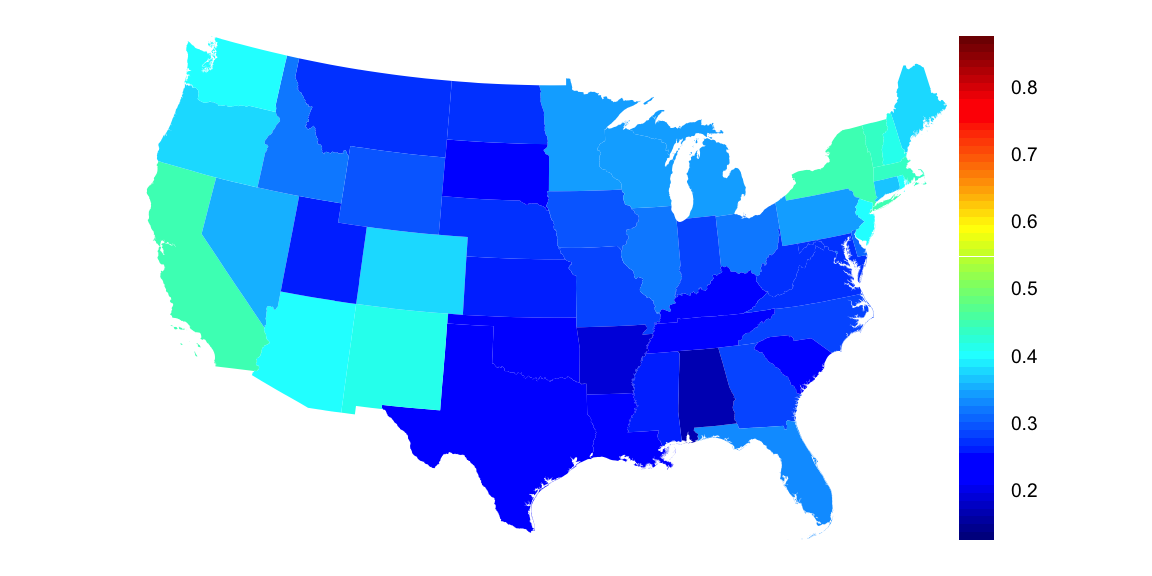
\includegraphics{MRP-vignette-firstmap}
\end{figure}

\section{The Full Model}
\label{sec:full-model}

In this section we demonstrate the use of the high-level arguments to \texttt{mrp()} for fitting more complex models with more data including intercepts strata not present in the population, additional group-level predictors, and transformations in the data.

The full model includes intercepts for poll (the data combine several polls), for region (states are grouped into regions), state-level predictors such as religious attendance and democratic vote share in previous elections, and interactions between the cross-classifying strata. The interface to supply or create this data and modify the regression formula are intuitive to use.

\subsection{Modifying Population Strata}
\label{sec:modify-popul-strata}

We would like to separate the estimation data by poll, but in general the population data will be the same across polls. To remove a stratification dimension, subtract it from the initial formula by adding this argument:
\begin{Schunk}
\begin{Sinput}
R> population.formula= . ~ . - poll
\end{Sinput}
\end{Schunk}

In the case where population arrays may differ across polls, such as polls over time with contemporaneous census values, the current method would require duplicating the census data across all polls for which it is the same and creating a factor of name and levels corresponding to those of \texttt{poll}.

\subsection{Joining Predictors and Transforming Data}
\label{sec:join-pred-transf}

the \texttt{add} argument is a powerful way to add predictors by left-joining (“merging”) other data.frames onto the prepared flattened cross-classified data. In this case we have state-level predictors -- a few that are used in the analysis and several others; and a set that are used only in the display -- but they are simple to join on matching keys in same-named columns. The \texttt{Statelevel} data.frame has a column `state' with factor levels matching those in the prepared data. 

Two common transformations are used in the data for this example: making a continuous group-level predictor out of the categorical one by rescaling it, and making an additional categorical variable by the interaction of other ones that are already included as cross-classifying strata.

Both types of additional data are provided in a \texttt{list}:
\begin{Schunk}
\begin{Sinput}
R> add=list(
     Statelevel,
     Regions,
     expression(z.age <- rescale(age)),
     expression(age.edu <- interaction(age,edu)))
\end{Sinput}
\end{Schunk}

\subsection{Specifying the Multilevel Regression Formula}
\label{sec:spec-mult-regr}

Finally, we need to adjust the multilevel regression formula. By default, \emph{MRP} will build a simple model for only intercepts by each stratum indicated in the main formula. We want to include all of those, but also the state-level predictors and possibly varying slopes in some of them as well. Again we use the dot to indicate what has already been included.

\begin{Schunk}
\begin{Sinput}
R> mr.formula= .~.+ (1|region) + (1|age.edu) + z.age + p.relig.full + p.kerry.full
\end{Sinput}
\end{Schunk}

\subsection{Re-fitting with existing data}
\label{sec:re-fitting-with}

The same updating of the formula is used in the event that you want to re-run or extend an existing analysis and modify its formula using the \texttt{mr()} method.

\subsection{Full Model \texttt{mrp()} Call}
\label{sec:full-model-call}

\begin{Schunk}
\begin{Sinput}
R> mrp.statelevel <- mrp(yes.of.all~
                         state+f.race+age+edu+poll,
                         data=marriage.data,
                         population=mrp.census,use="weighted2008",
                         population.formula=.~.-poll,
                         add=list(
                           Statelevel,
                           mrp.regions,
                           expression(age.edu <- interaction(age,edu))
                           ),
                         mr.formula=.~.+(1|region)+ (1|age.edu)+
                          p.relig.full+p.kerry.full
                         )
\end{Sinput}
\end{Schunk}
